\documentclass{article}
\usepackage[utf8]{inputenc}
\usepackage{natbib}
\usepackage{graphicx}

\title{Providing empirical estimates for the geostatistical characterization of subsurface hydraulic properties}
\author{falk.hesse }
\date{September 2021}

\begin{document}


\section{Results and discussion}

In the following, we will present and discuss the results of analyzing our data set. To that end, we will focus on statistical properties of the estimated variogram parameters. These are in particular the length scale, vertical and horizontal anisotropy, the nugget as well as potential shape parameters of the variogram model function. In addition, we will investigate and compare how different model functions are able to describe empirical variogram data. Since some variogram models have more parameters, i.e., degrees of freedom, we will investigate whether these additional degrees of freedom result in better fitting performance.


\subsection{Comparison between different variogram model function}

Generally, the performance varied the most when no plateau was reached within the covered spatial range (e.g., the Belridge field, Belgian nuclear repository)


\subsection{Scale-dependency}

As we already discussed in the introduction, the scale dependency of hydraulic properties like the correlation length is a well-know phenomenon from the literature \citep{Neuman2003, Neuman2008, Colecchio2020}. In the first step, we therefore investigated this property within our data set by fitting a model function to the empirical variogram cloud and estimating the correlation length for all sites in the data set. 

\begin{figure}[ht]
    \includegraphics[width=0.45\textwidth]{fig/scatter_len_scale_aquifer.png}
    \includegraphics[width=0.45\textwidth]{fig/scatter_len_scale_soil.png}
    \caption{Log length scale vs. log maximum length for variogram models fitted to data from aquifers (left) soil (right). The used variogram model function was the Mat{\'e}rn model.}
    \label{fig:scatter_len_scale}
\end{figure}

Results confirmed this general trend both for the case of soil and aquifer variogram functions (see Figure \ref{fig:scatter_len_scale}). Using a log-log plot, we can clearly see an excellent linear relationship between the estimated correlation length and the maximum length scale in the data set. Within this work, the maximum length scale was defined as the largest distance between two observation points in the data set, typically two piezometer stations or observation wells.

The purpose of this paper is not to weigh in on the long-time discussion around the nature of scaling effects and to what extent hydraulic variables represent intrinsic physical properties or are introduced by virtue of the measurement process. However, it could be said that these data and in particular the striking smoothness of the scaling behavior, do provide substantial evidence for the notion that the length scale of variogram functions does not solely represent an intrinsic physical property of the medium but is also strongly impacted by the truncation effects induced by the measurement process.

\begin{figure}[ht]
    \includegraphics[width=0.995\textwidth]{fig/length_scale_scatter_matrix.png}
    \caption{Scatter matrix plot for the estimated log length scales using the Gaussian, the Exponential, the Spherical, the Mat{\'e}rn and the Stable model function.}
    \label{fig:scatter_matrix_len_scale}
\end{figure}

To further investigate the behavior of the estimated length scale, we also looked at the different estimates derived using different variogram models; namely the Gaussian, the Exponential, the Spherical, the Mat{\'e}rn and the Stable model function. Results showed an overall strong linear correlation between between the estimates for all investigated variogram models (see Figure \ref{fig:scatter_matrix_len_scale}). While the slope of the regression plot varied, the overall trend was the same regardless of the used model. This demonstrates that all models measure the same underlying property of the empirical variogram cloud. Besides this strong linear correlation, a noticeably number for sites resulted in strongly diverging estimates depending on the model. We looked at a number of these sites and in all investigated cases, we found an empirical variogram function which had not yet reached a clear plateau. This resulted in a low sensitivity during the fitting procedure, since only a portion of the expected full variogram behavior was present in the data set. The different variogram models therefore reacted differently when exposed to these data and provided sometimes strongly diverging estimates for those parameters most sensitivity to the long term behavior of the variogram function, namely the length scale and the variance. It should be noted that in the literature, there was a tendency to perform the fitting such that the plateau of the model function was reached with the given empirical variogram cloud. Within this study we did not enforce such a condition resulting in the observed divergence between the different models.

\begin{figure}[ht]
    \includegraphics[width=0.45\textwidth]{fig/kdeplot_len_scale_aquifer.png}
    \includegraphics[width=0.45\textwidth]{fig/kdeplot_len_scale_soil.png}
    \caption{Kernel-density estimate of the residuals around the regression line of the data presented in Figure \ref{fig:scatter_len_scale} for aquifers (left) soil (right).}
    \label{fig:kdeplot_len_scale}
\end{figure}

To analyse the behavior of the scale dependency in more detail, we performed a kernel-density estimation for the residuals around regression line presented in Figure \ref{fig:scatter_len_scale}. The results showed a similar behavior for both aquifers and soils \ref{fig:kdeplot_len_scale}. In both cases, we saw that most estimated length scales were concentrated at around 1/10th of the maximum length scale with a noticeable uncertainty around that. This value coincides well with the empirical rule of thumb provided by Neuman. Apart from this center of mass, both aquifers and soils show estimated length scale that are larger than the maximum length scale present in the data set, a finding that is not explainable by a truncating process. These length scale estimates exceeding the maximum length scale are not only substantially less common, their estimated value is also much less certain. This is due to the fact that only a portion of the overall empirical behavior could be used for the fitting process making the fitting procedure less stable.

\begin{figure}[ht]
    \includegraphics[width=0.45\textwidth]{fig/kdeplot_len_scale_aquifer.png}
    \includegraphics[width=0.45\textwidth]{fig/kdeplot_len_scale_soil.png}
    \caption{Scatter plot of length scales determined for aquifers using a Mat{\'e}rn model function vs. using a Gaussian (left) and en Exponential (right) model function.}
    \label{fig:different_models_len_scale}
\end{figure}

All the above results present the length scale determined by fitting a Mat{\'e}rn variogram function to the empirical variogram cloud. To investigate the possible impact of different variogram functions on the estimation procedure, we also used the Gaussian and Exponential model and compared the results with each other. This comparison shows a very high degree on correlation between the different model functions. These comparisons show the generality of the presented results.

It should be noted that the distributions presented in Figure \ref{fig:kdeplot_len_scale} represent the uncertainty of a length scale estimate given a maximum length scale as a predictor. The are therefore a natural choice for the prior distribution of a Bayesian approach to variogram parameter estimation. Using a parametric approach, we can provide the following analytical expression for this uncertainty 

This linear model for the log correlation length was

$$
    log \lambda = 0.99722 log \Lambda - 2.2173,
$$ 

with $\Lambda$ being the aforementioned overall length scale.

These estimates depend of the used data set as well as the which may change over time. However, any practitioners can use the data set and the scripts presented here and redo the analysis to check its results as well as adapt them to their needs and applications.


\subsection{Anisotropy}

After having described the scale dependency of the correlation length, we will look at the ansiotropy of these estimates. As it is well known, subsurface anisotropy is well pronounced between the vertical and horizontal direction but is often assumed to be negligible between     9j  the two horizontal direction.

\begin{figure}[ht]
    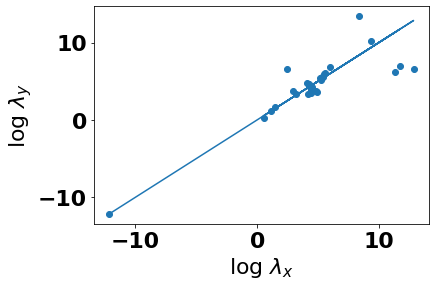
\includegraphics[width=0.45\textwidth]{fig/anisotropy_y_scatter.png}
    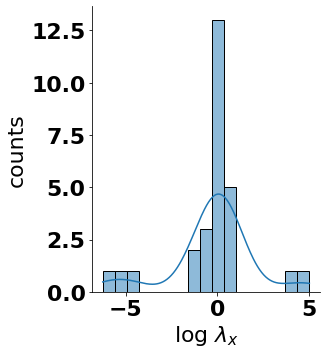
\includegraphics[width=0.45\textwidth]{fig/anisotropy_y_kde.png}
    \caption{Scatter plot of both main horizontal length scales determined for aquifers using a Mat{\'e}rn model function (left) a kernel-density estimate of the residuals around the diagonal.}
    \label{fig:anisotropy_y}
\end{figure}

Let us start with anisotropy in the horizontal direction. Results showed a strong linear relationship between the estimated log length scales in both directions (labeled $\lambda_x$ and $\lambda_y$ in Figure \ref{fig:anisotropy_y} left). The scatter is centered around the diagonal line, which is to be expected since the $x$ and $y$ directions are arbitrarily chosen and do not reflect and geological properties that could induce a meaningful difference between the two. Using the same procedure as above, we can also estimate the distribution around that center diagonal (see Figure \ref{fig:anisotropy_y} right). In general, this estimate is based on significantly fewer data points (n=27) and is therefore less reliable compared to the density estimates presented above. As a result a parametric model could be used to estimate the prior uncertainty. Given the tailing observable in \ref{fig:anisotropy_y}, a distribution with long tails like the $t$-distribution could be an acceptable match.

\begin{figure}[ht]
    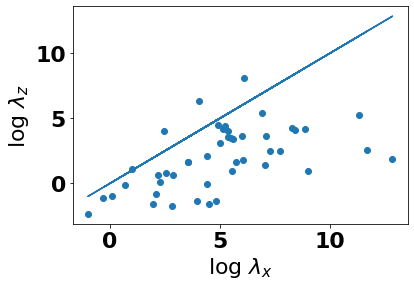
\includegraphics[width=0.45\textwidth]{fig/anisotropy_z_scatter.png}
    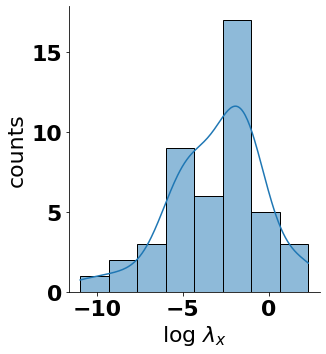
\includegraphics[width=0.45\textwidth]{fig/anisotropy_z_kde.png}
    \caption{Scatter plot of horizontal and vertical log length scales determined for aquifers using a Mat{\'e}rn model function (left) and a kernel-density estimate of the residuals around the diagonal (right).}
    \label{fig:anisotropy_z}
\end{figure}

Let us now look at the anisotropy between the vertical and horizontal directions. This anisotropy is known to be strongly pronounced due to the geological processes like sedimentation. Our results confirm this anisotropy with some notable exceptions (see Figure \ref{fig:anisotropy_z} left). Overall, the number of sites used for this estimation was substantially larger compared to the above case of horizontal anisotropy, with an overall number of $n=48$ sites being used. This number represents only sites in aquifers but could be increased if sites from soil variograms would be included. Since their numbers are overall small $n=4$, we performed no analysis for this group alone.

One of the most surprising results was the number of cases where the estimated vertical length scale is larger than the estimated horizontal length scale (see Figure \ref{fig:anisotropy_z} right). They are almost all caused by sites where the estimated length scale was larger than the maximum length scale. This indicates that it may be in part caused by the resulting uncertainty in the estimation procedure. It is consequently not clear whether these results should be used for the derivation of a prior distribution. If they were to be included, the resulting distribution shows again a long-tailed bell curve behavior. Like in the case of the horizontal anisotropy, we performed a parametric fitting procedure using the t-distribution (see Figure \ref{fig:anisotropy_z} right).


\subsection{Nugget value}

The next variogram parameter we estimated was the nugget parameter. This parameter describes the variance at the lag value of zero, ie., how much do measurements differ that are taken at effectively the same location. Such differences are often interpreted to represent either measurement errors or unresolved variations in the measurement variable below the measurement scale.

To investigate the behavior of the nugget parameter, we estimated its value using the Mat{\'e}rn model function and fitted it against our collected data set. For the analysis, we normalized the value of the nugget against the variance, making sure its value was between $0$ and $1$. We excluded cases where the normalized nugget was equal or larger than one since these represented case where the fitting procedure didn't converge. 

\begin{figure}[ht]
    \includegraphics[width=0.45\textwidth]{fig/nugget_aquifer_matern_kde.png}
    \includegraphics[width=0.45\textwidth]{fig/nugget_soil_matern_kde.png}
    \caption{Kernel-density estimate of the estimated nugget values for aquifer (left) and soil (right) sites. The used variogram model was the Mat{\'e}rn model.}
    \label{fig:nugget_matern}
\end{figure}

Results showed a somewhat similar behavior for the estimated distribution of nugget values for both aquifer and soil sites.  In general, most nugget values were close to $0$ in both cases indicating a small or negligible measurement error or sub-scale variabilities. Regardless, a substantial portion of the estimated nugget values were found above the value of $0.5$ meaning that large uncertainties are present in many data sets. Such higher values for the nugget were more common for data sets from soil sites leading to a bi-model behavior of the resulting density estimates. It should be noted that our soil data set was smaller compared to the aquifer data set ($n=71$ and $n=215$ for soil and aquifer sites, respectively). 

It should be noted that the kernel-density estimate presented in Figure \ref{fig:nugget_matern} is not a suitable representation of a prior density since it is not bounded by the interval between $0$ and $1$. Any parametric model function that is to be fitted against the sample should, therefore, be chosen to honor both these boundaries and the general behavior indicated in the kernel-density estimate. In Figure \ref{fig:nugget_matern}, we choose the Beta distribution but other models like the truncated log-normal distribution may be viable candidates as well.

\begin{figure}[ht]
    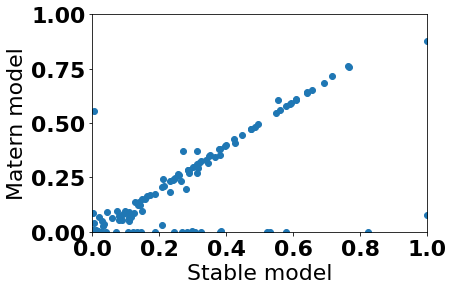
\includegraphics[width=0.45\textwidth]{fig/nugget_scatter_matern_stable.png}
    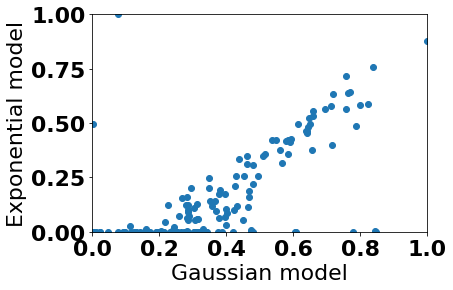
\includegraphics[width=0.45\textwidth]{fig/nugget_scatter_gaussian_exponential.png}
    \caption{Scatter plot of the estimated nugget values for the Mat{\'e}rn model vs. the Stable model (left) and Gaussian model vs. the exponential model (right). All data were draw from aquifer sites.}
    \label{fig:nugget_scatter}
\end{figure}

To investigate how the nugget value differed between the variogram model functions, we also compared their respective estimates. Our results showed a strong linear correlation between the estimated nugget of the Mat{\'e}rn model and the Stable model (see Figure \ref{fig:nugget_scatter} left), which shows the similarity between both model functions. On the other hand, plotting the estimated nugget of the Gaussian model vs. the Exponential model shows pronounced differences between the two (see Figure \ref{fig:nugget_scatter} right). This is due to the different behavior of these two models for small lag values. Wheres the Exponential model exhibits a steep gradient, the Gaussian model is essentially flat in this region. The different nugget values is therefore an artifact of the fitting procedure which tries to compensate for this difference through adjusting the nugget value. This demonstrates that prior distributions for this value are model specific and cannot in general be transferred between different mode functions. 

Estimated nugget values of the Spherical model showed the highest correlation with the nugget values of the Exponential model but low correlation with nugget values of all other investigated variogram model functions (data not shown). This is due to the similar behavior of the Spherical model and Exponential model at small lags showing again the relationship between this near-origin behavior of the model function and the ability of the nugget to compensate for any possible mismatch between the empirical variogram and the behavior of the model function. Although all shown results were derived using aquifer sites only, using data from soil sites did lead to the same results.



\subsection{Shape parameter}

Many common variogram model functions like the exponential and the Gaussian model are well defined by specifying the length scale, the variance and the nugget value. There is, however, a class of variogram model functions that feature an additional degree of freedom. In the following,we will call this additional parameter the shape parameter. 

In case of the well-known Mat{\'e}rn function, this value is known as the roughness parameter $\nu$, since its value is directly related to the roughness of the resulting spatial random field. This relationship is such that a low value means a high roughness, with the minimum value of $\nu=0.5$ resulting in a random field that has no derivatives whatsoever. A Mat{\'e}rn model function with such a low value of $\nu=0.5$ is mathematical identical to the exponential model function. On the other extreme, a very high value of $\nu \rightarrow \infty$ resulting in an extremely smooth field with an infinite number of derivatives. A Mat{\'e}rn model function with such a high value of $\nu=0.5$ is mathematical identical to the Gaussian model function.

\begin{figure}[ht]
    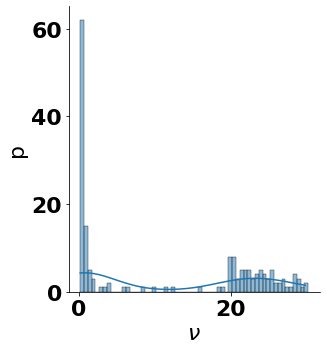
\includegraphics[width=0.45\textwidth]{fig/nu_aquifer_matern_kde.png}
    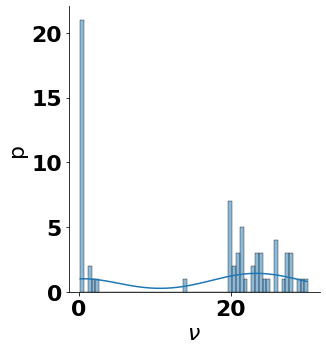
\includegraphics[width=0.45\textwidth]{fig/nu_soil_matern_kde.png}
    \caption{Kernel-density estimate of the estimated roughness parameter $\nu$ of the Mat{\'e}rn variogram model function for aquifer (left) and soil (right) sites.}
    \label{fig:nu_matern}
\end{figure}

Our results show a very pronounced bi-modal behavior of the resulting frequency distribution of $\nu$ values. This behavior is very similar for both aquifer and soil sites. The first peak of the estimated density corresponds well with a $\nu \approx 0.5$ indicating that an exponential model function would perform with similar accuracy in these case. On the other hand, the second peak is concentrated around $\nu \approx 25$. Although the Mat{\'e}rn function only converges to the Gaussian function in the limit of $\nu \rightarrow \infty$, it should be noted that for values of $\nu>10$, both functions become almost indistinguishable. The roughness parameter loses its sensitivity for higher values meaning that it barely changes the behavior of the function anymore. This means that a Gaussian model function would be able to similarly describe these cases very well.

These results indicate a number of things. First, despite the roughness parameter spanning a significant range, most of its values fall into two intervals, both of which can be approximated well with a more common model function, namely the exponential and Gaussian function. Second, the number of cases where a Gaussian model function would be a good fit is larger than expected. Due to its high smoothness, the Gaussian model function is sometimes considered unrealistic. This assessment is not supported by our findings at least from a simple fitting perspective. Finally, the Mat{\'e}rn model function is a relevant model function since it may not be clear in advance which classic function, i.e., the Gaussian or the exponential, provides a better performance. 

\begin{figure}[ht]
    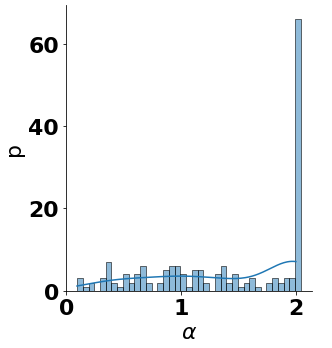
\includegraphics[width=0.45\textwidth]{fig/nu_aquifer_stable_kde.png}
    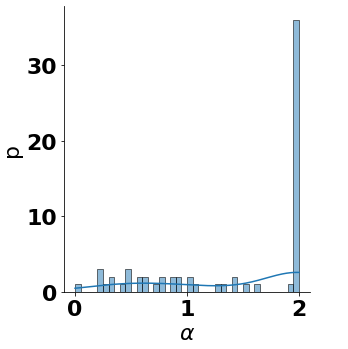
\includegraphics[width=0.45\textwidth]{fig/nu_soil_stable_kde.png}
    \caption{Kernel-density estimate of the estimated shape parameter $\alpha$ of the Stable variogram model function for aquifer (left) and soil (right) sites.}
    \label{fig:nu_stable}
\end{figure}

In the next step, we analyzed the data set using the Stable variogram model function. Our results show again a very pronounced bi-modal of the resulting frequency distribution of the shape parameter $\alpha$ (see Figure \ref{fig:nu_stable}). It should be noted that the shape parameter $\alpha$ is defined between $0$ and $2$. The overall similarity shows the strong relationship between the two shape parameters of the Mat{\'e}rn and the Stable mode functions. One difference is that the behavior of the shape parameter $\alpha$ is very similar for both aquifer and soil sites.

\begin{figure}[ht]
    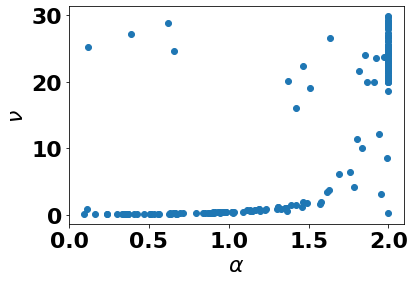
\includegraphics[width=0.45\textwidth]{fig/shape_parameter_aquifer_scatter.png}
    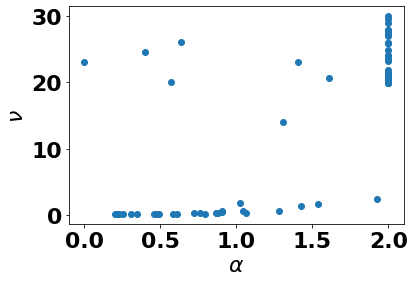
\includegraphics[width=0.45\textwidth]{fig/shape_parameter_soil_scatter.png}
    \caption{Scatter plot of the estimated shape parameter values for aquifer (left) and soil (right) sites.}
    \label{fig:shape_parameter}
\end{figure}

To better understand the relationship between the shape parameter $\nu$ of the Mat{\'e}rn model and the shape parameter $\alpha$ of the Stable model function, we performed a regression analysis for those sites where both model functions provided a fit. Our results show a very similar behavior for both aquifer and soil sites (see Figure \ref{fig:shape_parameter}). As can be seen, the scatter plot shows the most points in the scatter plot fall into two distinct correlations between $\nu$ and $\alpha$. First, for small values of $\nu$, representing an exponential-like behavior of the Mat{\'e}rn function, we see a linear correlation between the two. For high values of $\nu$, representing a Gaussian-like behavior of the  Mat{\'e}rn function, we see a nearly vertical behavior of the correlation. The latter is caused by the truncation behavior of the Stable model which is confined between values of $0$ and$2$. This means that the range of $\nu$ values, representing a Gaussian-like behavior, gets mapped into a very small interval of $\alpha$ values close to $2$.

In general, we can draw two conclusions from this observation. First, the shape parameter $\alpha$ of the Stable model is indeed very similar the roughness value $\nu$ of the Mat{\'e}rn model and can therefore be interpreted as a roughness parameter as well. Second, the confined parameter range of the Stable model is not a drawback from a practical point of view since the sensitivity of the Mat{\'e}rn model becomes really low for larger values of $\nu$. In fact, from a numerical perspective, this limitation of the parameter range is helpful since it improves the performance of an optimization algorithm necessary for the fitting procedure. Although this study does not aim to investigate this issue in detail, we did indeed observe a much higher numerical stability of the Stable model compared to the Mat{\'e}rn model. This stability is true both in terms of the number of steps necessary to find an acceptable fit between the model function and the empirical variogram function as well as in terms of the number of sites for which optimal parameters could be found in the first place. So although the name of this model is derived from the Stable distribution \citep{Wackernagel2003}, it also coincidentally describes its numerical behavior.

One thing that stood out from the data sets being used was the general lack of data for short lags. Most of these data sets were generated from observation networks that followed a regular grid layout. This make sense to maximize the coverage of the necessarily limited observation points. It is, however, problematic from a variogram estimation procedure. A good compromise would be to arrange at least some of the observation points in a logarithmic fashion \citep{Mueller2021}. 



%%%%%%%%%%%%%%%%%%%%%%%%%%%%%%%%%%%%%%%%%%%%%%%%%%%%%%%%%%%%%%%%%%%%%%%%%%%%
\bibliographystyle{plainnat}
\bibliography{ref}

\end{document}